\documentclass[showkeys, prb, reprint]{revtex4-1}

%%%%%%%%%%%%%%%%%%%%%%%%%%%%%%%%%%%%%%%
% -- Preamble: Packages and config -- %
%%%%%%%%%%%%%%%%%%%%%%%%%%%%%%%%%%%%%%%

% UTF8 encoding
\usepackage[utf8]{inputenc}
\usepackage{bbold}
\usepackage{amsmath}

% Graphics and path to graphics
\usepackage{graphicx}
\graphicspath{ {figures/} }
\usepackage{subcaption}

% Colors, especially for highlighting and editing
\usepackage[usenames, dvipsnames]{color}

%%%%%%%%%%%%%%%%%%%%%%%%%%%%%%
% -- Aliases and commands -- %
%%%%%%%%%%%%%%%%%%%%%%%%%%%%%%

\renewcommand{\d}{\delta}       % Dirac delta
\newcommand{\F}{\mathcal{F}}    % Free energy Functional
\renewcommand{\l}{\left}        % Quick left
\renewcommand{\r}{\right}       % Quick right
\newcommand{\f}{\frac}          % Quick fraction
\newcommand{\Z}{\mathcal{Z}}    % GC partition function
\newcommand{\D}{\mathcal{D}}    % Swirly D for path integrals
\newcommand{\fphi}{\tilde{\phi}}% Fourier space phi
\newcommand{\fh}{\tilde{h}}     % Fourier space h
\newcommand{\fxi}{\tilde{\xi}}  % Fourier space xi
\newcommand{\A}{\rho_A}         % Density of species A
\newcommand{\B}{\rho_B}         % Density of species B
\newcommand{\ham}{\mathcal{H}}  % Hamiltonian (classical)
\newcommand{\q}{\mathbf{q}}     % Phase space coordinates
\newcommand{\p}{\mathbf{p}}     % Phase space moment 

% Plane wave + and -
\newcommand{\pwp}{e^{\frac{i\mathbf{p}\cdot\mathbf{q}}{\hbar}}}
\newcommand{\pwm}{e^{-\frac{i\mathbf{p}\cdot\mathbf{q}}{\hbar}}}

% Classical Trace
\newcommand{\trace}[1]{\mathrm{Tr}\left[ #1 \right]}

% Average
\newcommand{\mean}[1]{\left\langle #1 \right\rangle}

% Integral
\newcommand{\integrate}[1]{\int \mathrm{d}#1\,}

% Lazy tilde
\newcommand{\til}{\tilde}

\begin{document}

%% Front (Top really...) Matter

\title{Improvements to the  Binary Phase Field Crystal Model}
\author{Nathan Smith}
\affiliation{McGill Department of Physics}
\author{Nikolas Provatas}
\affiliation{McGill Department of Physics}
\date{\today}

\begin{abstract}

[Abstract here]

\end{abstract}

\keywords{nucleation, growth, phase field crystal}

\maketitle

%% Body

%%%%%%%%%%%%%%%%%%%%%%%%
\section{Introduction} %
%%%%%%%%%%%%%%%%%%%%%%%%

% Thesis introduction outline: https://student.unsw.edu.au/introductions

% 1) State the general topic and give some background

The study of alloys in materials physics is a pursuit of incredibly broad
impact, affecting industries as diverse as those dealing with commercial
materials such as steel and aluminium alloys to nano-fabrication and
optoelectronics. Understanding of alloy properties can be difficult due to
their strong dependence on microstructure which forms through non- equilibrium
processes during their manufacturing. \textit{In situ} measurements of
microstructure formation, especially at the atomic level, are rarely feasible.

A broad spectrum of theoretical and numerical techniques have been successful
at predicting microstructure formation. In particular the Phase Field Crystal
(PFC) technique has been successful in describing microstructure formation on
diffusive time scales and atomic length scales at high temperatures where other
techniques including Kinetic Monte Carlo, Diffusive MD and Accelerated
Molecular Dynamics can fail.

% 2) Outline the current situation

In this paper, we'll focus on extending a branch of binary PFC theory known as
the binary {\it XPFC} model --where the "X" in XPFC signifies a class of PFC
models  constructed to controllably simulate a robust range of metallic and
non-metallic crystal symmetries compared to the original PFC models. PFC binary
models have been successful in describing a broad selection of phenomena in
binary alloys.  These successes include eutectic and dendritic solidification
\cite{ELDER07}, the Kirkendall effect \cite{ELDER11_KIRKENDALL, LU15}, solute
drag \cite{GREENWOOD12}, clustering and precipitation \cite{FALLAH12, FALLAH13,
FALLAH13_AlCu_experiment}, colloidal ordering in drying suspensions
\cite{GANAI13}, epitaxial growth and island formation \cite{ELDER10_NANOISLAND,
LU16}, and ordered crystals \cite{ALSTER17} to name a few. 

The PFC theory is derived from Classical Density Functional Theory (CDFT) and
as such, it can be considered a simplified density functional theory.  In
practice, two different variants of the PFC theory are used, as alluded to
above: the original model developed by Elder \textit{et al} \cite{ELDER07} and
the Structural Phase Field Crystal (XPFC) model developed by Greenwood
\textit{et al.} \cite{GREENWOOD11_BINARY}.

The original model was the first PFC theory of binary alloys and contains some
important physical properties of binary alloys. However, it is a very reduced
form of CDFT and it therefore lacks completeness in its ability to describe
binary alloys. Specifically, the original model uses an expansion in
concentration that is actually a density difference not a concentration, and
the model has a limited ability to describe a realistic or robust range of
phase diagrams. The original model also uses a very simplified correlation
kernel which limits its ability to describe a variety of crystal lattice
structures.

The XPFC model is an improvement that ameliorates the above problems. The
concentration is left unexpanded allowing for construction of realistic global
phase diagrams instead of local expansions. More significantly, the XPFC model
provides a phenomenology for modelling two-point correlation functions that
succeeded in describing solidification of a variety of lattice structures, as
well as transformations between different crystal lattices. Simplifications of
the multi-modal approach first introduced with the XPFC formalism has been used
to produce hexagonal, square, kagome, honeycomb, rectangular and other lattices
in 2 dimensions \cite{MKHONTA13}.

% 3) Evaluate the current situation and identify a gap

In introducing its phenomenology for modelling correlation functions, the
binary XFPC theory tacitly assumes that there is some preferred structure at
high concentration and some other structure preferred at low concentration.
This assumption can be limiting in situations that have a specific crystalline
structure at intermediate concentrations, such as materials with a syntectic
phase diagram. At the syntectic point a solid of intermediate concentration
solidifies along the interface between a solute rich and solute poor liquid.
The XPFC model also assumes no long wavelength correlations in the
concentration field which, in practice, means the model has an ideal free
energy of mixing.  This is another limitation of the XPFC model because the
enthalpy of mixing is not generally zero for alloy systems.

% 5) State the research goals and aims

The goal of the current research is threefold: The first two goals are to
present two important improvements to the binary XPFC theory. The first
improvement is a more general phenomenology for modelling pair correlation
functions of a binary material. The second improvement is to extend the free
energy of mixing beyond ideality to account for circumstances when the enthalpy of
mixing is not negligible. The third goal is to use the new XPFC model derived
herein to the elucidate the multi-step nucleation process seen in certain
diffusion-limited systems including gold and silver nanoparticles \cite{LOH17}.

%%%%%%%%%%%%%%%%%%%%%%%%%%%%%%%%%
\section{Binary PFC Background} %
%%%%%%%%%%%%%%%%%%%%%%%%%%%%%%%%%

We begin with a binary classical density functional theory. The intrinsic free
energy functional can be approximated by expanding about a reference mixture
with number densities $\rho_A^0$ for component A and $\rho_B^0$ for component
B,
%
\begin{align}
    \label{binary_cdft_free_energy}
    \beta\F[\A, \B] &= \sum_{i=A, B} \int \mathrm{d}r 
        \,\rho_i(r) \ln\l(\f{\rho_i(r)}{\rho_i^0}\r) 
        - (1 - \beta\mu_i^0)\Delta\rho_i(r)\\
    &- \f{1}{2} \sum_{i,j=A, B} \Delta\rho_i(r) \ast C^{(2)}_{ij}(r, r^\prime) 
        \ast \Delta\rho_j(r^\prime). \nonumber
\end{align}
%
Where,
\begin{description}
    \item[$\mu_i^0$] is the reference chemical potential of component $i$,
    \item[$\Delta\rho_i$] is the deviation from the reference density,
    \item[$C^{(2)}_{ij}(r, r^\prime)$] is the direct correlation function
        of the reference mixture and,
    \item[$\ast$] denotes an integral over repeated arguments.
\end{description}

It is convenient to change variables to a dimensionless total density, $n(r)$
and local concentration, $c(r)$,
%
\begin{gather}
    n(r) = \f{\Delta \rho}{\rho_0} = \f{\Delta\A + \Delta\B}{\A^0 + \B^0} \\
    c(r) = \f{\B}{\rho} = \f{\B}{\A + \B}.
\end{gather}
%
Scaling out a factor of the total reference density, $\rho_0$ we can break the
free energy functional in these new variables into three parts,
%
\begin{equation}
    \label{binary_total_free_energy}
    \f{\beta\F[n, c]}{\rho_0} = \f{\beta\F_{id}[n]}{\rho_0} 
        + \f{\beta\F_{mix}[n, c]}{\rho_0}
        + \f{\beta\F_{ex}[n, c]}{\rho_0},
\end{equation}
%
where, $\F_{id}$, $\F_{mix}$ and $\F_{ex}$ are the ideal, mixing and excess
free energies respectively. These are defined as,
%
\begin{gather}
    \label{binary_ideal}
    \f{\beta\F_{id}}{\rho_0} =
        \int \mathrm{d}r \,\l\lbrace (n(r) + 1)\ln(n(r) + 1) 
        - (1 - \beta\mu^0)n(r) \r\rbrace \\
    \label{binary_mixing}
    \f{\beta\F_{mix}}{\rho_0} =
        \int \mathrm{d}r \,\l\lbrace (n(r) + 1)\l( 
            c\ln\l(\f{c}{c_0}\r) + (1-c)\ln\l(\f{1-c}{1-c_0}\r) \r)\r\rbrace, 
\end{gather}
%
where we have introduced $\mu^0=\mu_A^0+\mu_B^0$ as the total chemical
potential of the reference mixture, and $c_0 = \B^0 / \rho_0$ as the reference
concentration. Assuming that the local concentration $c(r)$ varies over much
longer length scales than the local density $n(r)$, the excess free energy term
becomes  
%
\begin{align}
    \label{binary_excess}
    \f{\beta\F_{ex}[n, c]}{\rho_0}
        = &-\f{1}{2} n(r) \ast \l[ 
            C_{nn}(r, r^\prime) \ast n(r^\prime) 
          + C_{nc}(r, r^\prime) \ast \Delta c(r^\prime)\r] \\
        &-\f{1}{2} \Delta c(r) \ast \l[
            C_{cn}(r, r^\prime) \ast n(r^\prime) 
          + C_{cc}(r, r^\prime) \ast \Delta c(r^\prime)\r], \nonumber
\end{align}
%
where we have introduced  and $\Delta c(r) = c(r) - c_0$ as the deviation of the 
concentration from the reference.  The $n-c$ pair correlation introduced in the 
excess free energy are,
%
\begin{align}
    C_{nn} &= \rho_0\l(c^2 C_{BB} + (1 - c)^2C_{AA} + 2c(1-c)C_{AB}\r) \label{binaryCs}\\
    C_{nc} &= \rho_0\l(c C_{BB} - (1 - c) C_{AA} + (1 - 2c)C_{AB}\r) \\
    C_{cn} &= C_{nc} \\
    C_{cc} &= \rho_0\l(C_{BB} + C_{AA} - 2 C_{AB}\r)
\end{align}
%

Differences in the various simplified binary PFC theories stem from differing
approximations of the terms in the free energy stated in equations 
\ref{binary_ideal}, \ref{binary_mixing} and \ref{binary_excess}.

%%%%%%%%%%%%%%%%%%%%%%%%%%%%%%%%%%%%%%%%%%%%%%%%%%%%%
\section{Original Binary Phase Field Crystal Model} %
%%%%%%%%%%%%%%%%%%%%%%%%%%%%%%%%%%%%%%%%%%%%%%%%%%%%%

In the original simplified binary PFC theory, all terms in the free energy are
expanded about $n(r) = 0$ and $c(r) = c_0$ (ie., about their reference states).
For the ideal free energy this results in a polynomial truncated to fourth
order,
%
\begin{equation}
    \label{ideal_expansion}
    \f{\beta\F_{id}[n]}{\rho_0} = \integrate{r}
    \l\lbrace \f{n(r)^2}{2} - \eta\f{n(r)^3}{6} + \chi\f{n(r)^4}{12} \r\rbrace.
\end{equation}
%
The linear term in the expansion is dropped by redefining $n$ about its average
and we have added the fitting parameters $\eta$ and $\chi$ to fit the free
energy away from the reference parameters. If we assume for simplicity of
demonstration $c_0 = 1/2$, the free energy of mixing becomes a simple fourth
order polynomial as well,
%
\begin{equation}
    \f{\beta\F_{mix}[n, c]}{\rho_0} = \integrate{r} \l\lbrace
       2\Delta c(r)^2 + \f{4\Delta c(r)^4}{3}
    \r\rbrace.
\end{equation}
%
Linear couplings to $n(r)$ are dropped by assuming, as we already have, that
the concentration field varies on a much longer length scale than the total
density and noting that the total density is defined about its average. This
argument can also be applied to the linear couplings to $n(r)$ in the excess free
energy term, which then leaves only the $C_{nn}$ and $C_{cc}$ terms. Finally, these
two terms are approximated with a gradient expansion of the form,
%
\begin{gather}
    C_{nn}(r, r^\prime) = \l( C_0 + C_2 \nabla^2 + C_4 \nabla^4 + \dots\r)
        \d(r - r^\prime), \\
    C_{cc}(r, r^\prime) = \l(\epsilon + W_c \nabla^2 + \dots\r)
        \d(r - r^\prime).
\end{gather}
%
The expansion parameters, $C_0, C_2,$ and $C_4$ are all dependent on
temperature and concentration. We are required to expand $C_{nn}$ to fourth
order because the peak of the direct correlation function in Fourier space is
the driving force for solidification.  The concentration field is correlated
over a longer length scale implying that only the short wavevectors are
important in $C_{cc}$ so we can expand just to quadratic order, effectively
treating $c$ as in the traditional Cahn-Hilliard theory.

Gathering terms, the resulting free energy functional for the original
simplified binary PFC model\footnote{The orignal simplified binary PFC model
was expressed using slightly different variables. We expand in $\Delta c(r)$
here to facilitate comparison with other theories} is,
%
\begin{align}
    \f{\beta\F[n, c]}{\rho_0} &= \integrate{r} \l\lbrace 
        \f{1}{2} n(r) \l( 1 - C_0 - C_2 \nabla^2 - C_4\nabla^4 \r) n(r)
      - \eta\f{n(r)^3}{6} + \chi\f{n(r)^4}{12} \r\rbrace \\
    &+ \integrate{r} \l\lbrace
        \f{1}{2} \Delta c(r) \l( 4 - \epsilon - W_c\nabla^2 \r) \Delta c(r) 
      + \f{4 \Delta c(r)^4}{3} \r\rbrace. \nonumber
\end{align}
%

The strength of the original simplified binary PFC model is that is retains
most of the important physics of binary alloys in a very reduced theory. For
instance, the simplified model is capable of describing the equilibrium phase
diagrams of both eutectic alloys and materials with a solid state spinodal /
liquid minimum.  Supplied with a diffusive equation of motion, the simplified
model can model an impressive diversity of dynamic phenomena including eutectic
growth \cite{ELDER07}, solute segregation \cite{STOLLE14}, dendritic growth
\cite{ELDER07}, epitaxial growth \cite{ELDER10_NANOISLAND, LU16} and crack
formation \cite{HU17}.

The major limitation of the original simplified model is that the gradient
expansion of the density-density correlation function gives only a crude
control over the crystal structures that can be formed. In fact, as this theory
only controls a single peak in Fourier space it can only solidify into the BCC
phase.

A second limitation of the original simplified model is that it is local in
concentration. This means that realistic phase diagrams from 0 to 100\%
concentration cannot be produced, only local phase diagrams around the
reference concentration\footnote{Indeed, the original model concentration was
in fact a density difference, not true concentration.}. The limited
concentration range is problematic for comparing to experimental phase
diagrams. To obtain relatable and testable results, a major motivation for
binary XPFC and this work, we require the entire free energy of mixing term in
eqution \ref{binary_mixing}.

%%%%%%%%%%%%%%%%%%%%%%%%%%%%%%%%%%%%%%%%%%%%%%%%%%%%%%%%%%%%%%%%
\section{Original Binary Structural Phase Field Crystal Model} %
%%%%%%%%%%%%%%%%%%%%%%%%%%%%%%%%%%%%%%%%%%%%%%%%%%%%%%%%%%%%%%%%

The binary structural phase field crystal theory (XPFC) seeks to remedy the two
short comings of the original simplified model. That is, it seeks to reproduce
a variety of crystal lattice structure and to construct  phase diagrams of a
range of concentrations. We'll begin with a derivation of the theory and
compare with the original model.

First, the ideal free energy is expanded in precisely the same manner resulting
in the same fourth order polynomial,
%
\begin{equation}
    \f{\beta\Delta\F_{id}[n]}{\rho_0} = \integrate{r}
        \l\lbrace \f{n(r)^2}{2} - \eta \f{n(r)^3}{6} + \chi\f{n(r)^4}{12}
        \r\rbrace. \tag{\ref{ideal_expansion} revisited}
\end{equation}
%
The free energy of mixing is left unexpanded but an overall scale $\omega$ is
added to fit the mixing term away from the reference concentration,
%
\begin{equation}
    \f{\beta\F_{mix}[n, c]}{\rho_0} =
        \integrate{r} \l\lbrace \omega (n(r) + 1)\l( 
            c\ln\l(\f{c}{c_0}\r) + (1-c)\ln\l(\f{1-c}{1-c_0}\r) \r)\r\rbrace. 
\end{equation}
%
This unexpanded free energy of mixing will lead to more accurate global phase
diagrams. The excess free energy is approximated using similar assumptions as
in the original model (linear couplings are dropped), but the density-density
correlation function, $C_{nn}$, is not expanded. Instead, Greenwood \textit{et
al} all assumed that the $k=0$ mode of the concentration-concentration
correlation function was zero leaving only the quadratic term in the expansion,
%
\begin{equation}
    C_{cc}(r, r^\prime) = \d(r - r^\prime)W_c \nabla^2.
\end{equation}
%
Grouping terms together, the complete free energy functional for the binary
XPFC model is,
%
\begin{align}
    \f{\beta\Delta\F[n, c]}{\rho_0} &= \integrate{r} \l\lbrace
        \f{1}{2} n(r) \l(1 - C_{nn}(r, r^\prime)\r) \ast n(r^\prime)
        - \eta \f{n^3}{6} + \chi \f{n^4}{12} \r\rbrace \\
        &+ \integrate{r}\l\lbrace
            \f{W_c}{2}\l\vert \nabla c(r) \r\vert^2 + \omega f_{mix}(r)
            \r\rbrace. \nonumber
\end{align}
%
Where $f_{mix}(r)$ is the local free energy density of mixing,
%
\begin{equation}
    f_{mix}(r) = \l(n(r) + 1\r)\l( 
            c(r)\ln\l(\f{c(r)}{c_0}\r) + (1-c(r))\ln\l(\f{1-c(r)}{1-c_0}\r) \r).
\end{equation}
%

The density-density correlation function, $C_{nn}$, is left unexpanded in 
Fourier space but assumed to have a specific phenomenological form,
%
\begin{equation}
    \label{eq:xpfc_corr}
    C_{nn} = \zeta_A(c) C_{AA}(r, r^\prime) 
           + \zeta_B(c) C_{BB}(r, r^\prime),
\end{equation}
%
where $\zeta_A(c)$ and $\zeta_B(c)$ are interpolation functions, assigned the forms
%
\begin{gather}
    \zeta_A(c) = 1 - 3c^2 + 2c^3 \\
    \zeta_B(c) = \zeta_A(1 - c).
\end{gather}
%
by Greenwood \textit{et al.}

The remaining elemental correlation functions $C_{AA}$ and $C_{BB}$ are modelled
using the general XPFC model for correlation functions, which we describe
subsequently.

%%%%%%%%%%%%%%%%%%%%%%%%%%%%%%%%%%%%%%%%%
\subsection{XPFC Correlation Functions} %
%%%%%%%%%%%%%%%%%%%%%%%%%%%%%%%%%%%%%%%%%

The key insight made by the XPFC model is that the density-density
correlation function can be modelled in such a way as to control the crystal
lattice structure formed under solidification and to target different structures at
different concentrations, and temperatures. Originally delineated for pure
systems, the XPFC method for constructing correlation functions is strongly
influenced by the methods developed by Ramakrishnan. In particular this means
that we need a model correlation function that controls the values specifically
at the reciprocal lattice vector positions. We can achieve this with Gaussian
peaks centred at the reciprocal lattice vector positions,
%
\begin{equation}
    \tilde{C}(k) = \sum_{\alpha} e^{-\f{T}{T_0}}
        e^{ - \f{(k - k_\alpha)^2}{2\sigma_\alpha^2}}
        \label{XPFC_C2}
\end{equation}
%
Where the index $\alpha$ runs over sets of point group symmetry-equivalent
reciprocal lattice vectors, $k_\alpha$ is the length of the reciprocal lattice
vectors in $\alpha$ and $\sigma_\alpha$ is the width of the peak. Temperature
dependence of the correlation peaks in the is achieved through the prefactors
$e^{-T / T_0}$ give the correct temperature scaling of the amplitudes at
temperatures much higher than the Debye temperature\footnote{The original XPFC
works used a phenomenological prefactor $e^{-\sigma^2 / C}$, where $\sigma$
was considered a model temperature parameter and $C$ a constant. That choice
was inspired by harmonic analysis in the solid phase and the Debye-Waller
factor.} as discussed by \cite{ALSTER17}.

The primary advantages of the XPFC model are two fold: they produce realistic
phase diagrams and they model a variety of crystalline lattices. While the
former is relatively cosmetic the latter allows for the examination of
genuinely novel systems in comparison with the original simplified model. For
example, the binary XPFC model has been used to study peritectic systems
\cite{GREENWOOD11_BINARY}, ordered crystals \cite{ALSTER17},
dislocation-assisted solute clustering and precipitation \cite{FALLAH12,
FALLAH13} and solute drag \cite{GREENWOOD12}. It is noteworthy, that the above
works on clustering have been validated experimentally in binary and ternary
alloys.

Unfortunately, by assuming that the $k=0$ mode of the
concentration-concentration correlation function is zero, the XPFC model
restricts its free energy of mixing to an ideal model of mixing. This model of
mixing includes only entropic contributions to the free energy. In the solid
state, this means that the sole driving force for phase separation is elastic
energy as the enthapy of mixing is always zero. This inhibits the modelling a
variety of binary alloy systems, for instance both monotectic and syntectic
systems cannot be modelled without a negative enthalpy of mixing. 

A second disadvantage of the present XPFC model is that the phenomenological
form for the correlation function as seen in equation \ref{eq:xpfc_corr}
implicitly assumes that there are well defined structures at $c=0$ and $c=1$.
This works well for modelling eutectic systems for example, but does not work
very well when we expect a solid phase at intermediate concentration. These
shortcomings are the motivation for the improvements developed in this paper
which are presented in the following section.

%%%%%%%%%%%%%%%%%%%%%%%%%%%%%%%%%%%%%%%%%%%%%%%%%%%%%%%%%%%%%%%%
\section{Improvements to the Binary Phase Field Crystal Model} %
%%%%%%%%%%%%%%%%%%%%%%%%%%%%%%%%%%%%%%%%%%%%%%%%%%%%%%%%%%%%%%%%
\label{sec:improvements}

In this section we look at two improvements to the binary XPFC theory. The
improvements, as previously alluded to, are to first, extend the free energy of
mixing in the XPFC model to one with an enthalpy of mixing and to second,
generalize the phenomenological for of the two-point correlation function in
binary alloys.

%%%%%%%%%%%%%%%%%%%%%%%%%%%%%%%%%%%%%%%%%%%
\subsection{Adding an Enthalpy of Mixing} %
%%%%%%%%%%%%%%%%%%%%%%%%%%%%%%%%%%%%%%%%%%%

Extending the free energy of mixing beyond ideal mixing is achieved by removing
the assumption made by Greenwood \textit{et al.} in deriving the binary XPFC
model that the concentration-concentration correlation function has no $k=0$
mode. This is the same approach taken in the original PFC model, though here we
keep the ideal mixing term unexpanded as in the original XPFC alloy model.
Specifically, the correlation function is expanded as,
%
\begin{equation}
    C_{cc}(r, r^\prime) = \d(r - r^\prime)
        \l(\omega\epsilon + W_c\nabla^2 + \cdots\r),
\end{equation}
%
where $\epsilon$ is a parameter that is possibly temperature dependent. This
form results in a free energy functional of the form,
%
\begin{align}
    \f{\beta\Delta\F[n, c]}{\rho_0} &= \integrate{r} \l\lbrace
        \f{1}{2} n(r) \l(1 - C_{nn}(r, r^\prime)\r) \ast n(r^\prime)
        - \eta \f{n^3}{6} + \chi \f{n^4}{12} \r\rbrace \\
        &+ \integrate{r}\l\lbrace
            \f{W_c}{2}\l\vert \nabla c(r) \r\vert^2 + \omega f_{mix}(r)
            \r\rbrace, \nonumber
\end{align}
%
where the local free energy density of mixing, $f_{mix}$ is now,
%
\begin{equation}
    f_{mix}(r) = \l(n(r) + 1\r)\l(
            c(r)\ln\l(\f{c(r)}{c_0}\r)
          + (1-c(r))\ln\l(\f{1-c(r)}{1-c_0}\r) \r)
          + \f{1}{2} \epsilon (c - c_0)^2.
\end{equation}
%
For simplicity the temperature dependence of the parameter $\epsilon$ is taken
to be linear about a spinodal temperature $T_c$,
%
\begin{equation}
    \label{eq:spinodal_model}
    \epsilon(T) = -4 + \epsilon_0(T - T_c).
\end{equation}
%
The resulting model has a free energy of mixing that is equivalent to the
regular solution model and, as such, it makes a clear connection to a well used
model elsewhere in material science. The regular solution model also supplies
the essential physics of a non-negligible enthalpy of mixing. 

%%%%%%%%%%%%%%%%%%%%%%%%%%%%%%%%%%%%%%%%%%%%%%%%%%%%%%%%%%%%%%
\subsection{Generalizing the Two-Point Correlation Function} %
%%%%%%%%%%%%%%%%%%%%%%%%%%%%%%%%%%%%%%%%%%%%%%%%%%%%%%%%%%%%%%

To establish a general phenomenology for modelling density-density correlation
functions in alloys, note that the density-density correlation function has the
form of a linear combination of interpolating functions in concentration,
$\zeta(c)$, multiplied by bare correlation functions $C(r, r^\prime)$ of
individual components,
%
\begin{equation}
    C_{nn}(r, r^\prime; c) = \sum_i \zeta_i(c) C_i(r, r^\prime)
\end{equation}
%
where the index $i$ is, for the moment, an arbitrary label. For example, in the
exact theory that emerges from the original alloy CDFT theory (equation
\ref{binaryCs}), we use the labels $\lbrace AA, AB, BB\rbrace$ to enumerate the
interpolation functions, 
%
\begin{gather}
    \zeta_{AA}(c) = \rho_0 (1 - c^2), \\
    \zeta_{AB}(c) = \rho_0 c (1 - c ), \\
    \zeta_{BB}(c) = \rho_0 c^2.
\end{gather}
%
This suggests the following new definition that we introduce herein to
generalize the density-density correlation function for a binary alloy: Use the
labels $i$ to enumerate the set of crystal structures known to manifest
themselves in an alloy system. The correlation functions, $C_i(r, r^\prime)$
are then direct correlation functions that model the crystal structure $i$ and
the associated interpolation functions $\zeta_i(c)$ define the range of
concentrations over which these correlations are valid. In principle,
$\zeta_i(c)$ can also be temperature dependent, although we do not consider
that case in this thesis.

As a simple example, if we wanted to construct a model of the silver-copper
eutectic alloy system, we might start with some model correlation function for
pure silver, $C_\alpha(r, r^\prime)$, and for pure copper, $C_\beta(r,
r^\prime)$. These two structures, the silver rich $\alpha$ phase and the copper
rich $\beta$ phase, are the only two relevant crystalline phases in the system,
so to build the full density-density correlation function we just need to
choose interpolating functions for each phase. Following Greenwood \textit{et
al} for example, we might choose,
%
\begin{gather}
    \zeta_\alpha(c) = 1 - 3c^2 + 2c^3, \\
    \zeta_\beta(c) = 1 - 3 (1 - c)^2 + 2(1 - c)^3.
\end{gather}
%
To model the $\alpha$ and $\beta$ correlation functions we use the original
XPFC formalism for modelling bare correlation functions (i.e. equation
\ref{XPFC_C2}). The $\alpha$ and $\beta$ phase are both FCC
\cite{SUBRAMANIAN93} so we can use an FCC model for the correlation function as
in \cite{GREENWOOD10}.

%%%%%%%%%%%%%%%%%%%%%%%%%%%%%%%%%%%%%%%%%%%%%%%%%%%
\section{Equilibrium Properties of Binary Alloys} %
%%%%%%%%%%%%%%%%%%%%%%%%%%%%%%%%%%%%%%%%%%%%%%%%%%%

These two changes to the XPFC formalism extend the possible systems we can
study. In this section we'll explore the equilibrium properties of the improved
XPFC free energy functional specialized for three different material phase
diagrams: eutectic, syntectic and monotectic.

%%%%%%%%%%%%%%%%%%%%%%%%%%%%%%%%%%%%%
\subsection{Eutectic Phase Diagram} %
%%%%%%%%%%%%%%%%%%%%%%%%%%%%%%%%%%%%%

While previous PFC models have shown that elastic energy is a sufficient
driving force for eutectic solidification, our simplified regular solution XPFC
model allows for the examination of the role enthalpy of mixing can play in
eutectic solids.  For instance, Murdoch and Schuh noted that in nanocrystalline
binary alloys, while a positive enthaply of segregation can stabilize against
grain growth via solute segregation at the grain boundary, if the enthaply of
mixing becomes too large this effect can be negated by second phase formation
or even macroscopic phase separation\cite{MURDOCH13}. 

To specialize our simplified regular model to the case of the binary eutectic,
we must choose an appropriate model for the correlation function. Choosing an
$\alpha$ phase around $c = 0$ and $\beta$ phase around $c = 1$, we can recover
the pair correlation function used in the binary XPFC of Greenwood \textit{et
al.} with a particular choice of interpolations functions: 
%
\begin{align}
   \zeta_\alpha(c) &= 2c^3 - 3c^2 + 1 \\
   \zeta_\beta(c) &= \zeta_\alpha(1 - c).
\end{align}
%
Should we choose, for example, an $\alpha$ and $\beta$ phase with 2 dimensional
hexagonal lattices, differing only by lattice constants, we can produce a phase
diagram like that in Fig. \ref{eutectic}. The phase diagram also depicts the
phase diagram of the metastable liquid below the eutectic point showing the
binodal and spinodal lines where the metastable liquid becomes unstable with
respect to phase separation. The spinodal line indicates an inflexion point in
the free energy of the metastable liquid where the liquid becomes fully
unstable with respect to phase separation whereas the binodal line indicates
the coexistance curve of the decomposed metastable liquid.

\begin{figure}[h]
    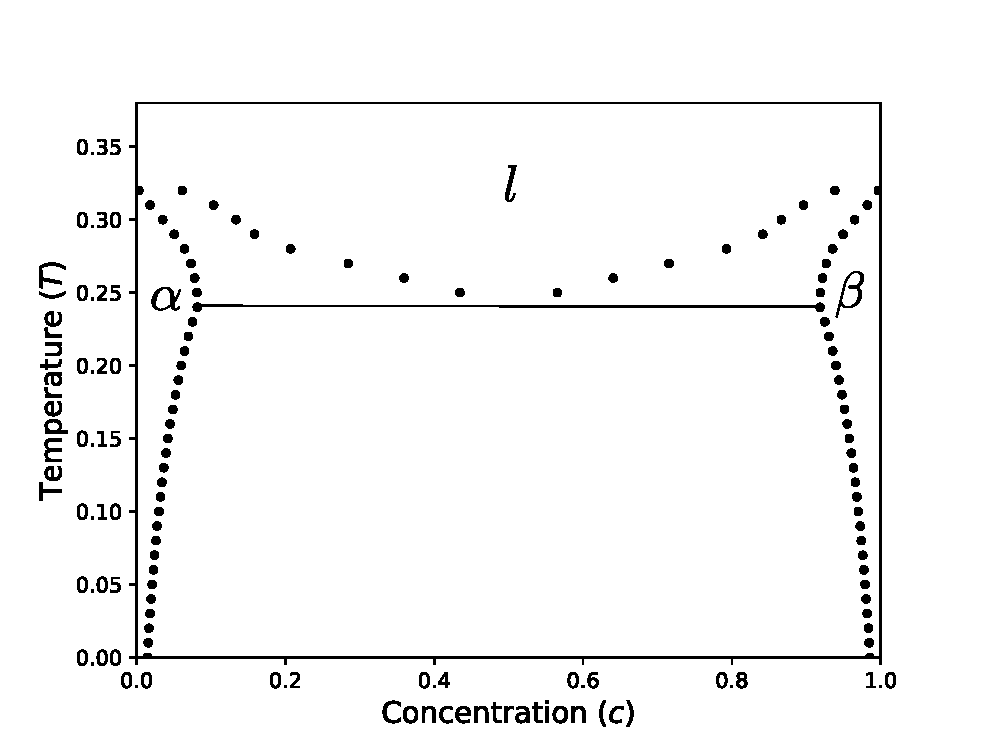
\includegraphics[scale=0.45]{eutectic}
    \caption[Eutectic Phase Diagram]{
        \label{eutectic} Eutectic phase diagram for triangle $\alpha$ and
        $\beta$ solid phases and $l$ denotes the liquid. The free energy
        parameters are $\eta = 2$, $\chi = 1$, $\omega=0.02$, $\epsilon_0 =
        26.6$ and $T_c = 0.15$. The parameters of the structure functions are
        $\sigma_{10\alpha} = \sigma_{10\beta} = 0.8$, $k_{10\alpha} = 2\pi$,
        $k_{10\beta} = 4\pi/\sqrt{3}$ and $T_0 = 1$. The horizontal line
        denotes the eutectic temperature.
    }
\end{figure}

It is noted that the phase diagram in Fig. \ref{eutectic} and in what follows
were done using the same approach that was used in numerous PFC literature
\cite{GREENWOOD11_BINARY}. The approach is as follows: a mode expansion for the
density is assumed for each crystal phases (zero amplitudes for the liquid
phase). For each  phase, an amplitude equation results, except in this case, it
is a function of amplitudes, average density {\it and} concentration. This
coarse grained free energy of each phase is then minimized with respect to the
amplitudes, leaving a free energy density for each phase that is a function
only of the average density and concentration. At this juncture, we simplify
matters by assuming that the average density is a constant for the system. We
then minimize the total free energy of the system with respect to
concentration, assuming a conserved total concentration field. This latter step
considers separately the coexistence of  (1) $\alpha$-liquid, (2)
$\beta$-liquid, (3) $\alpha$-$\beta$ over different temperature/concentration
ranges. Original code was developed to carry our these phase diagram
constructions, and implemented using \texttt{Julia} \cite{JULIA},
\texttt{Maxima.jl} \cite{MAXIMAJL} and the \texttt{Maxima} symbolic computation
engine \cite{MAXIMA}.  

%%%%%%%%%%%%%%%%%%%%%%%%%%%%%%%%%%%%%%
\subsection{Syntectic Phase Diagram} %
%%%%%%%%%%%%%%%%%%%%%%%%%%%%%%%%%%%%%%

Our improved XPFC model also allows for the study of a variety of invariant
binary reactions that, to date, have not been studied using phase field crystal
models. One such reaction is the syntectic reaction. 

The syntectic reaction, $l_1 + l_2 \rightarrow \alpha $, consists of
solidification at the interface of two liquids. We can achieve this with our
model by setting the spinodal temperature, $T_c$, in equation
\ref{eq:spinodal_model} sufficiently high and producing a density-density
correlation function that is peaked at a concentration below the spinodal. This
can be done by choosing a single interpolation function to be a window 
function that is centered about an intermediate concentration, $c_\alpha$ of 
the solid phase, $\alpha$. One obvious choice is, 
%
\begin{equation}
  \zeta(c) = e^{- \f{(c - c_\alpha)^2}{2 \alpha_c^2}}
\end{equation}
%
The resulting correlation function for a hexagonal lattice in a syntectic alloy
in two dimensions becomes, 
%
\begin{equation}
  \tilde{C}_{nn}(k; c) = 
    e^{-\f{(c - c_\alpha)^2}{2 \alpha_c^2}}
    e^{-\f{T}{T_0}} 
    e^{-\f{(k - k^\prime)^2}{2\alpha^2}}
\end{equation}
%
A phase diagram that produces a syntectic reaction with an appropriate choice
of parameters can be seen in Fig. \ref{syntectic}.

\begin{figure}
	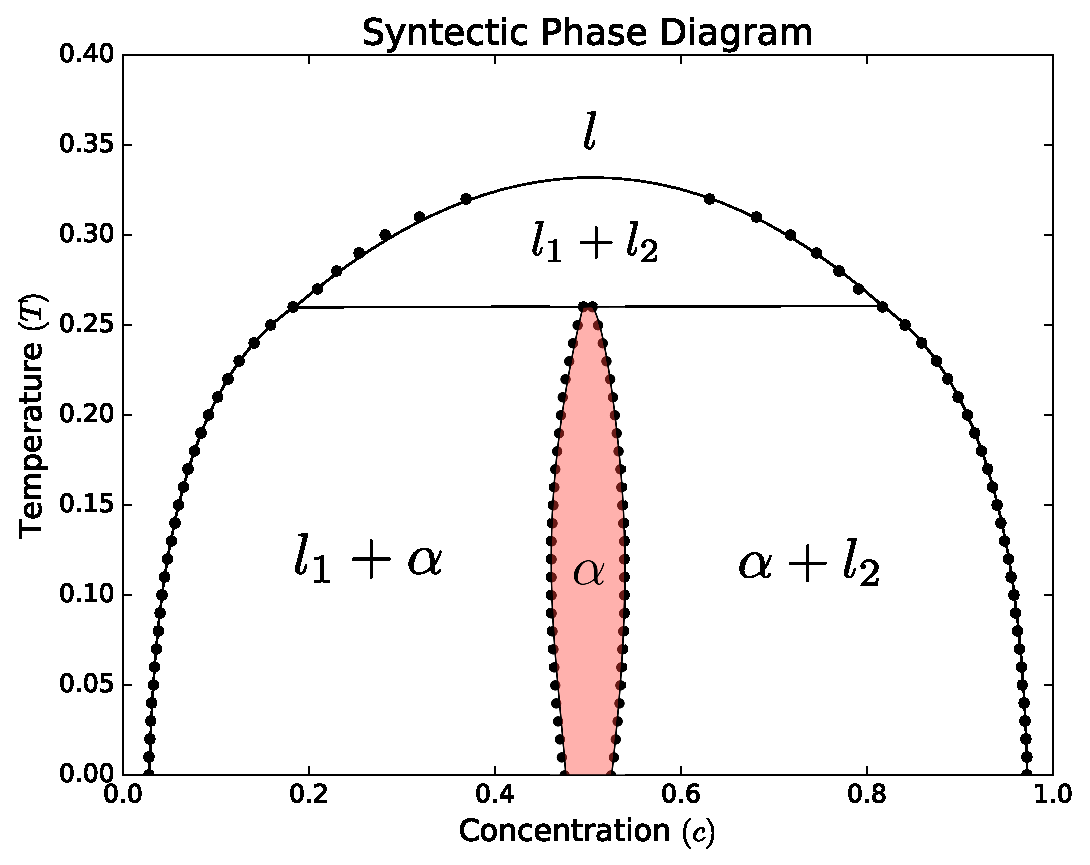
\includegraphics[scale=0.5]{syntectic.eps}
    \caption[Syntectic Phase Diagram]{
        \label{syntectic} Phase Diagram of Syntectic Alloy with a hexagonal
        solid phase $\alpha$. The free energy parameters are $\eta=2$,
        $\chi=1$, $\omega=0.3$, $\epsilon_0 = 10$ and $T_c=0.35$. The
        parameters for the structure function are $\alpha_{10\alpha} = 0.8$,
        $k_{10\alpha} = 2\pi$ and $T_0 = 1$. The horizontal line denotes the
        syntectic temperature.
    }
\end{figure}

%%%%%%%%%%%%%%%%%%%%%%%%%%%%%%%%%%%%%%%
\subsection{Monotectic Phase Diagram} %
%%%%%%%%%%%%%%%%%%%%%%%%%%%%%%%%%%%%%%%

The monotectic reaction is another invariant binary reaction that has not
previously been studied using PFC models. The monotectic reaction, $l_1
\rightarrow \alpha + l_2$, consists of decomposing liquid into a solute poor
solid and solute rich liquid. To model a monotectic using our improved XPFC
model we hypothesize a solid phase at $c=0$ and set the spinodal temperature
higher than the solidification temperature. To achieve this, we use a window
function peaked around $c = 0$,
%
\begin{equation}
    \chi_\alpha(c) = e^{-\f{c^2}{2\alpha_c^2}}.
\end{equation}
%
Again considering a simple hexagonal lattice for the $\alpha$ phase, we can
produce a phase diagram with a monotectic reaction with an appropriate choice
of parameters as in Fig. \ref{monotectic}.

\begin{figure}
	\includegraphics[scale=0.5]{monotectic.eps}
    \caption[Monotectic Phase Diagram]{
        \label{monotectic} Phase Diagram of Monotectic Alloy with hexagonal
        $\alpha$ phase. The free energy parameters are $\eta = 2$, $\chi=1$,
        $\omega=0.3$, $\epsilon_0 = 10$, $T_c = 0.35$ and $c_0 = 0.75$. The
        parameters for the structure function are $\alpha_{10\alpha} = 0.8$,
        $k_{10\alpha} = 2\pi$ and $T_0 = 1$ and the parameter for the window
        function is $\alpha_c = 0.4$. The horizontal line indicates the 
        monotectic temperature.
    }
\end{figure}

The improvements to the XPFC formalism made in this chapter not only reveal new
details in existing systems, but also model new systems that haven't been
explored with PFC methods before. They provide a general framework to explore
the landscape of other possible possible binary alloys with an emphasis that
the liquid free energy is a crucial element in this complete description. It is
also noteworthy that the approach introduced here is extendable in a
straightforward way to multi-component alloys if the interpolation functions
become multivariate functions of the concentrations.

%%%%%%%%%%%%%%%%%%%%%%%%%%%%%%%%%%%%%%%%%%%%%%%%%%%%%%%%%%%%%%%%%%%%
\section{Application to Precipitating Nanoparticles from Solution} %
%%%%%%%%%%%%%%%%%%%%%%%%%%%%%%%%%%%%%%%%%%%%%%%%%%%%%%%%%%%%%%%%%%%%

In this section we discuss applications of the improved binary XPFC model
introduced in section \ref{sec:improvements} to an application in
microstructure evolution.  We first begin with, we introduce  a
phenomenological set of equations of motion that describe solute and density
diffusion in the binary XPFC model. We then apply these to the examination of
the process of diffusion limited precipitation from solution.  Recent
experimental work on the precipitation of gold and silver nanoparticles
\cite{LOH17} and on the precipitation of calcium carbonate \cite{WALLACE13} has
demonstrated that the pathway to nucleation can deviate highly from the
approximations of Classical Nucleation Theory (CNT).  Specifically, both
experiments observe spinodal decomposition of the solution prior to nucleation
in the solute rich phase. In this chapter, we'll present early findings from
our new model that lend support for this dynamical behaviour and, additionally,
show that the growth behaviour post-nucleation may be more complex than usual
diffusive growth and coarsening typically observed.  To conclude we discuss
future applications both in the study of precipitation and other areas.

%%%%%%%%%%%%%%%%%%%%%%%%%%%%
\subsection{XPFC Dynamics} %
%%%%%%%%%%%%%%%%%%%%%%%%%%%%

To examine applications of our improvements to the XPFC model we begin by
considering equations of motion. Following \cite{GREENWOOD11_BINARY}, we use
conservative dynamics for both $n(x, t)$ and $c(x, t)$.
%
\begin{gather}
    \f{\partial n(x, t)}{\partial t} = 
        M_n \nabla^2\l(\f{\d \beta \Delta\F / \rho_0}{\d n(x, t)}\r) 
        + \xi_n(x, t), \\ 
    \f{\partial c(x, t)}{\partial t} = 
        M_c \nabla^2\l(\f{\d \beta \Delta \F / \rho_0}{\d c(x, t)}\r)
        + \xi_c(x, t),
\end{gather}
%
where $M_n$ and $M_c$ are the solute and density mobilities. The noise terms
$\xi_n(x, t)$ and $\xi_c(x, t)$ model thermal fluctuations. Their dynamics
follow the fluctuation-dissipation theorem, the theory of which is derived in
the Appendix \ref{appendix:noise}. These equations of motion are largely
phenomenological as, strictly speaking, there is no reason that the local
concentration should be conserved.  This conservation can be justified in the
limit that the total density does not deviate far from the reference. When this
is the case we have $c \equiv \B / \rho \approx \B / \rho_0$ which \textit{is}
conserved. For simplicity, we will carry out simulations in this paper in
this limit.

%%%%%%%%%%%%%%%%%%%%%%%%%%%%%%%%%%%%%%%%%%%%%%%%%%%%%%%%%%%%%%%%%
\subsection{Multi-Step Nucleation of Nanoparticles in Solution} %
%%%%%%%%%%%%%%%%%%%%%%%%%%%%%%%%%%%%%%%%%%%%%%%%%%%%%%%%%%%%%%%%%

% Supply some background on the problem and motivation

Many nanoparticle solutions are formed by precipitation from solution and their
size distribution (polydispersity index) is of key importance to their
application. Therefore, a precise understanding of the kinetic pathway of
precipitation is of crucial importance in designing synthesis techniques of
highly mono-disperse nanoparticles.

As stated above, recent experimental work has shown that precipitation from a
solution can follow a pathway vary different from that assumed by Classical
Nucleation Theory (CNT) \cite{LOH17, WALLACE13}. CNT assumes that, for binary
systems, changes in composition occur simultaneously to changes in order. In
contrast, these experimental findings suggest that in certain systems changes
in composition can precede changes in order via spinodal decomposition. While
there is some dispute about whether or not to call this process a non-classical
\textit{nucleation} pathway \cite{DAVEY13, GEBAUER11}, the observed pathway to
precipitation raises several questions about its classification, regardless of
semantics.

%%%%%%%%%%%%%%%%%%%%%%%%%%%%%%%%%%%%%%%%%%%%%%%%%%%%%%%%%%%%%%
\subsection{Classical and Non-classical Nucleation Theories} %
%%%%%%%%%%%%%%%%%%%%%%%%%%%%%%%%%%%%%%%%%%%%%%%%%%%%%%%%%%%%%%

% Discuss classical nucleation theory

In CNT, the rate of formation of post-critical can be written as an Arrhenius
equation,
%
\begin{equation}
    J = \f{\partial n^*}{\partial t} = A e^{-\beta\Delta G^{\ddagger}},
\end{equation}
where,
\begin{description}
    \item[$A$] is a constant prefactor,
    \item[$\Delta G^\ddagger$] is the Gibbs free energy of a critical nucleus
        and, 
    \item[$n^*$] is the number if critical nuclei.
\end{description}
% 
Following \cite{MYERSON04}, the probability of nucleation of a droplet of
volume $V$, $f_{nuc}(t)$, is then,
%
\begin{equation}
    f_{nuc}(t) = \mean{\f{N_{cry}}{N_{total}}} = 1 - e^{-J V t},
\end{equation}
%
where $N_{cry}$ and $N_{total}$ are the number of crystalline droplets and the
total number of droplets respectively.

% Discuss non-classical nucleation theory and the methods of reaction co-ordinates

CNT assumes that there is a single critical state which is specified by the
thermodynamic parameters of the target phase at a critical radius $R^*$. This
naive approach dramatically underestimate the time required to assemble a
critical nucleus due to its simplistic parametrization of the kinetic pathway
\cite{LUTSKO15, MYERSON04, MYERSON09}.

Improvements to CNT can be made to the model by increasing the parameter space
describing the nucleation process. Considering both radius and density of the
critical nucleus \cite{LUTSKO15} gives good agreement with nucleation of
globular proteins, for example. One problem with this approach is the selection
of appropriate parameters. There is no guarantee that a finite set parameters
will describe the kinetic pathway taken by a nucleus and if we are without a
fundamental technique for calculating the chosen parameters we have little way
of knowing if our theory is accurate or simply over-fit. In \cite{MYERSON09},
for example, nucleation data is fit to the functional form instead of using
calculated or otherwise measured parameters.

% Posit that field theory present an unbiased (un-parameterized) approach to nucleation

Statistical field theories such as the XPFC alloy model can help provide an
answer to this problem by taking an unbiased approach to nucleation process
within the context of CDFT.  The critical state, and entire kinetic pathway,
can be examined free of any particular parametrization. The equations of motion
can be integrated numerically for an ensemble systems and nucleation details
measured from the computed results.  Moreover, unlike other numerical
approaches to nucleation like molecular dynamics or formal density functional
theory, the PFC model can examine nucleation on diffusive time scales.

%%%%%%%%%%%%%%%%%%%%%%%%%%%%%%%%%%%%%%%%%%%%%%
\subsection{XPFC Modelling of Precipitation} %
%%%%%%%%%%%%%%%%%%%%%%%%%%%%%%%%%%%%%%%%%%%%%%

% Motivate a submerged spinodal phase diagram

To construct an appropriate free energy functional for a system analogous to
gold nanoparticles studied by Loh \textit{et al.} \cite{LOH17} we consider the
structure of its equilibrium phase diagram. Precipitation is indicative of a
simple liquid-solid coexistance curve. The presumed presence of spinodal
decomposition under certain circumstances indicates that is a metastable liquid
spinodal submerged beneath the liquid-solid coexistance curve \cite{DAVEY13}.
We assume that there must exist conditions under which the spinodal
decomposition of the metastable liquid phase occurs more rapidly than
nucleation directly from solution (ie., classical nucleation).

% Discuss the implementation of this phase diagram using our improvements

Producing a phase diagram in our XPFC model with these characteristics is very
similar to modelling a monotectic system with the exception that the spinodal
temperature $T_c$ must be low enough to hide the entire liquid spinodal below
the coexistance curve.  We will also centre the interpolation function
$\zeta_\alpha(c)$ about $c = 1$ so that the nanocrystalline solid $\alpha$ is
favoured at large concentration. The resulting density-density correlation
function for a 2 dimensional hexagonal precipitate would thus be,
%
\begin{equation}
    \label{eq:precip_corr}
    \tilde{C}_{nn}(k; c) = \exp\l\lbrace - \f{(c - 1)^2}{2\sigma_c^2}\r\rbrace
        \exp\l\lbrace \f{T}{T_0} \r\rbrace 
        \exp\l\lbrace - \f{(k - k_{10})^2}{2\sigma^2} \r\rbrace,
\end{equation}
%
where,
\begin{description}
    \item[$\sigma_c$] is the width of the interpolation function
        $\zeta_\alpha(c)$, which controls the solvent solubility in the
        precipitate in this case and,
    \item[$k_{10}$] is the length of the [10] reciprocal lattice vector of the
        preciptate in equilibrium.
\end{description}

An example phase diagram of a system with sample parameters in equation
\ref{eq:precip_corr} is shown in figure \ref{fig:precip_phase_dia}. The
metastable binodal (coexistence) and spinodal curves are depicted below the
coexistence curve.

\begin{figure}
    \centering	
    \includegraphics[scale=0.5]{solution.eps}
    \caption[Coexistance Phase Diagram with Metastable Spinodal]{
        \label{fig:precip_phase_dia} Phase Diagram of a Precipitating Solution
        with hexagonal $\alpha$ phase solid. The free energy parameters are
        $\eta = 2$, $\chi = 1$, $\omega=0.3$, $\epsilon_0=30$, $T_c = 0.15$ and
        $c_0 = 0.5$. The parameters for the correlation function from equation
        \ref{eq:precip_corr} are $\sigma = 0.8$, $k_{10} = 2\pi$, $T_0 = 1$ and
        $\sigma_c = 0.5$.
    }
\end{figure}

%%%%%%%%%%%%%%%%%%%%%%%%%%%%%%%%%%%%%%%%%%%%%%%%%%%%%%%%%%%%%%%%
\subsection{Dynamics of Precipitation: Results and Discussion} %
%%%%%%%%%%%%%%%%%%%%%%%%%%%%%%%%%%%%%%%%%%%%%%%%%%%%%%%%%%%%%%%%

% Describe with supporting figures the typical path way of precipitation.
 
We examined the precipitation process in a system that follows the XPFC model
with corresponding equilibrium phase diagram in figure
\ref{fig:precip_phase_dia}. The situation examined corresponded to a quench to
a temperature below the metastable spinodal curve. The spinodal curve marks an
inflection point in the liquid free energy meaning the metastable liquid
becomes fully unstable and decomposes into regions of differing concentration
as a result. A typical microstructure evolution sequence results for a typical
quench of a uniform solution of $c = 0.3$ from the liquid phase to a
temperature $T/T_0 = 0.07$ is shown in figure \ref{fig:precipitation}.
Frames (a)-(c) show the initial decmposition of the liquid, once below the
spinodal temperature, into two regions of high and low compositions. Frames
(d)-(f) show that once the concentration in the solute-rich regions of the
decomposed liquid occurs, nucleation of the solid phase begins to occur in
these confined liquid volumes. Once nucleated, the solid regions start/continue
to grow at the expense of the liquid phase. Finally, in frames (g)-(i), the
nucleated nanoparticles undergo growth and coarsening. This simulation is a
typical example where the nucleation of precipitates in preceded by spinodal
decomposition, which is consistent with the  the experimental findings
mentioned above for the nanoparticle and calcium carbonate systems \cite{LOH17,
WALLACE13}. While one simulation sequence is show here, this scenario was
typical of all ensembles we ran and from which we gathered statistics for the
data shown below. As mentioned above, we observed that once any solute-rich
regions crystallize, their growth is accelerated at the expense of
uncrystallized solute-rich regions. We refer to this phenomena as
\textit{sacrificial growth} (frames (d)-(f) in figure
\ref{fig:precipitation})). 
%
\begin{figure}
    \centering
    \begin{subfigure}[b]{0.3\columnwidth}
        \includegraphics[width=\textwidth]{initial}
        \label{fig:initial}
        \caption{}
    \end{subfigure}
    ~
    \begin{subfigure}[b]{0.3\columnwidth}
        \includegraphics[width=\textwidth]{early_spinodal}
        \label{fig:early_spinodal}
        \caption{}
    \end{subfigure}
    ~
    \begin{subfigure}[b]{0.3\columnwidth}
        \includegraphics[width=\textwidth]{devel_spinodal.png}
        \label{fig:devel_spinodal}
        \caption{}
    \end{subfigure}

    \vspace{0.25cm}
    \begin{subfigure}[b]{0.3\columnwidth}
        \includegraphics[width=\textwidth]{nucleation}
        \label{fig:nucleation}
        \caption{}
    \end{subfigure}
    ~
    \begin{subfigure}[b]{0.3\columnwidth}
        \includegraphics[width=\textwidth]{nucleation_and_sacrificial_growth}
        \label{fig:nucleation_and_growth}
        \caption{} 
    \end{subfigure}
    ~
    \begin{subfigure}[b]{0.3\columnwidth}
        \includegraphics[width=\textwidth]{sacrificalgrowth}
        \label{fig:sacrifical_growth}
        \caption{}
    \end{subfigure}
    
    \vspace{0.25cm}
    \begin{subfigure}[b]{0.3\columnwidth}
        \includegraphics[width=\textwidth]{crystalgrowth}
        \label{fig:crystalgrowth}
        \caption{}
    \end{subfigure}
    ~
    \begin{subfigure}[b]{0.3\columnwidth}
        \includegraphics[width=\textwidth]{crystalgrowth2}
        \label{fig:crystalgrowth2}
        \caption{}
    \end{subfigure}
    ~ 
    \begin{subfigure}[b]{0.3\columnwidth}
        \includegraphics[width=\textwidth]{crystalgrowth3}
        \label{fig:crystalgrowth3}
        \caption{}
    \end{subfigure}
    \caption[Stages of precipitation of nanoparticles from solution]{
        \label{fig:precipitation}
        Various stages of precipitation of nanoparticles from solution. All
        thermodynamic parameters are shared with figure
        \ref{fig:precip_phase_dia}. The initial condition is a uniform solution
        quenched abruptly to $T$ = 0.07. The initial condition has
        concentration $c = 0.3$ and relative density is set to $n = 0.05$. Mobilities
        $M_n$ and $M_c$ are set to 1 and $W_c$ is set to 3.0. Numerical
        parameters are grid spacing $\Delta x = 0.125$ on a 1024 by 1024
        lattice with time step size $\Delta t = 0.0025$. Sub-figures (a) - (c)
        show spinodal decomposition of the liquid into solute right and solute
        poor regions. Sub-figures (d) - (f) show nucleation of the solid and
        solid growth at the expense of liquid regions.  The remaining
        sub-figures show only nanoparticle growth and coarsening.
    }
\end{figure}
%

% Discuss the growth picture (hyper / hypo diffusive)
%
To quantify the phenomena shown in figure \ref{fig:precipitation}, we examine
the mean radius $\mean{R(t)}$ of solute-rich domains as a function of time, and
average the results over an ensemble of 120 quenches analogous to those shown in 
figure \ref{ig:crystalgrowth3}. Here we define the mean
radius as the square root of the mean area,
%
\begin{equation}
    \mean{R(t)} = \sqrt{\mean{A(t)}}.
\end{equation}
%
The results obtained are not expected to depend on the precise definition of
$R(t)$.

In purely diffusive growth the mean radius should scale as $\mean{R(t)} \sim
t^{1/2}$, while at the late steges of growth, where coarsening occurs, the
growth rate is expected to follow  $\mean{R(t)} \sim t^{1/3}$ dynamics.  In
figure \ref{fig:scaling} we plot $\langle R(t)\rangle$ on a log-log graph.
Lines corresponding to the diffusive growth exponent are also drawn for
comparison to numerical results. The data shows that for early times,
crystalline regions grow at a hyper-diffusive rate. 
%
\begin{figure}
    \centering
    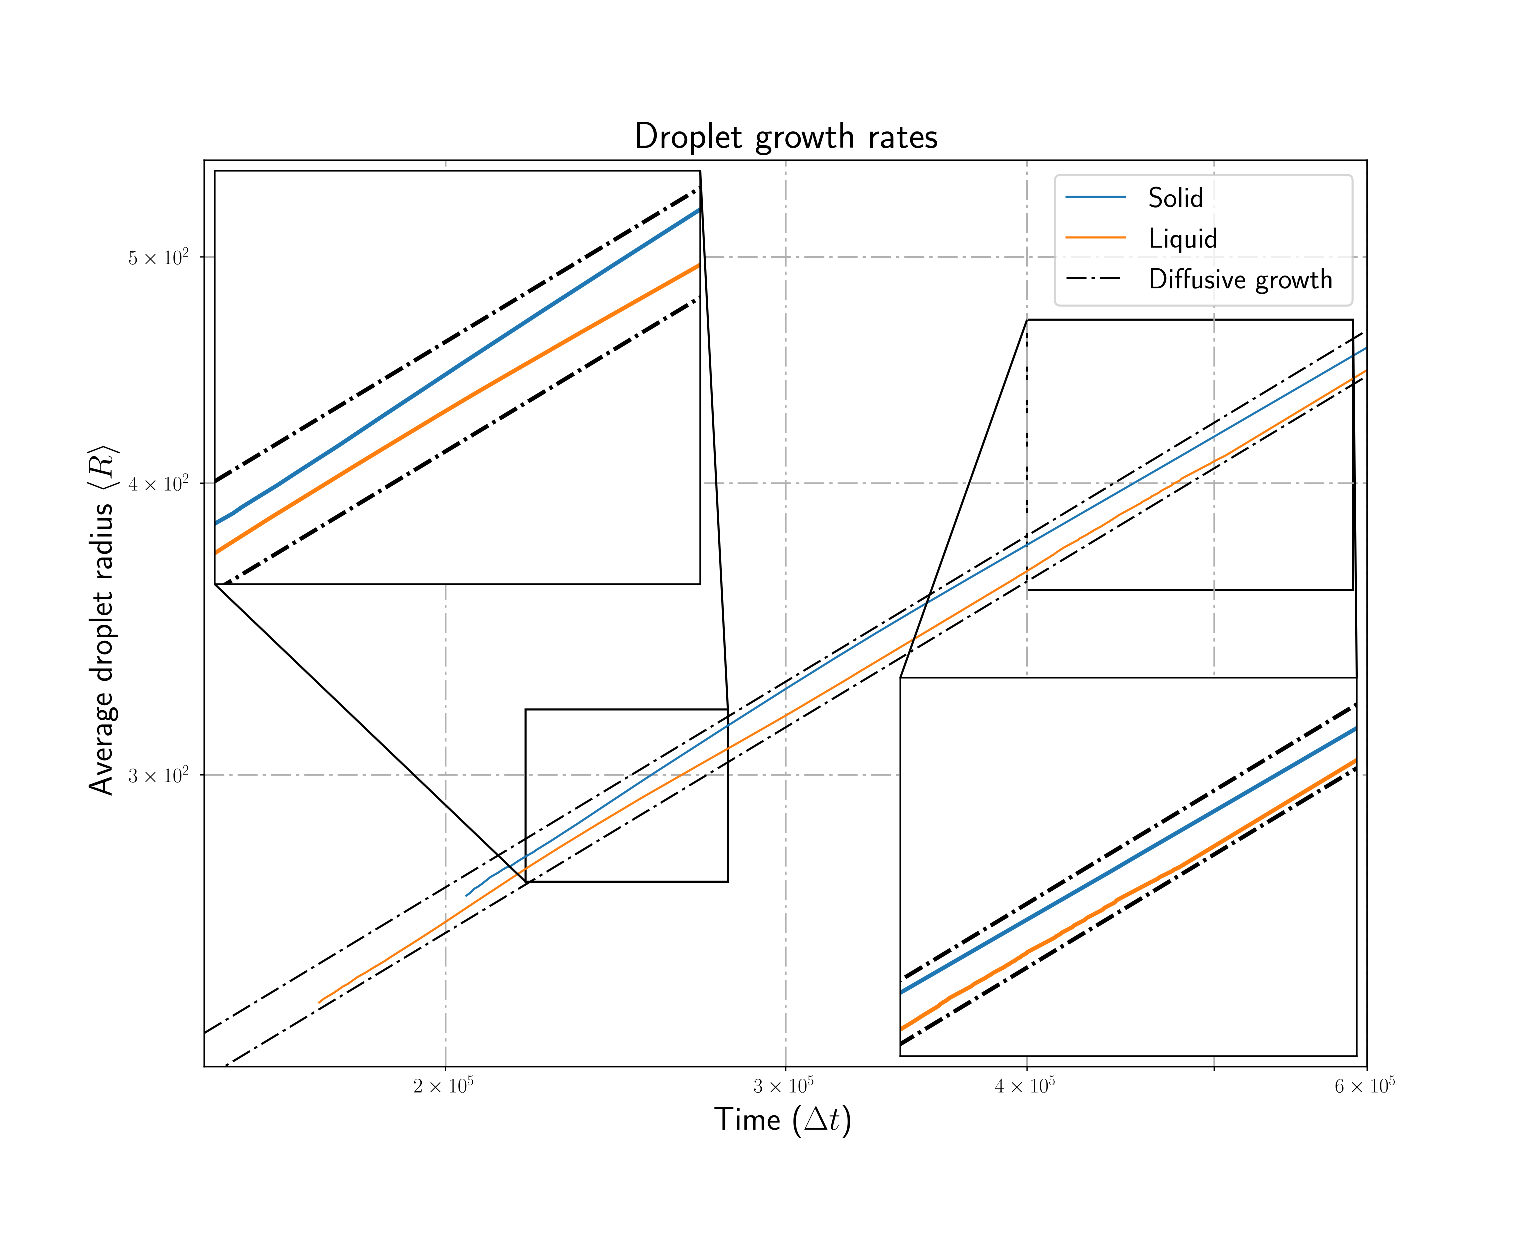
\includegraphics[width=\columnwidth]{scaling}
    \caption{
        \label{fig:scaling}
        Droplet growth $\langle R(t) \rangle$ Versus time. Black line show
        $\sim t^{1/2}$ growth. Insets show early hyper-diffusive growth
        of crystalline nanoparticles and late stage hypo-diffusive growth.
    }
\end{figure}
%
\noindent This decays to hypo-diffusive after uncrystallized regions have disappeared and
coarsening takes over the kinetics of precipitation.

% Discuss the nucleation picture (fraction of uncrystallized droplets)
% and compare with MYERSON for example

During sacrificial growth period referred to above, we observe that nucleation
is suppressed in the remaining uncrystallized solute-rich regions. When both
crystallized and uncrystallized solute-rich regions exist, solute is segregated
into crystallized regions because of the difference in chemical potential.
Constricted by surface tension and deprived of solute, these remaining droplets
have a far slower nucleation rate (thermodynamic driving force) than when no
crystallized regions exist. This can be seen more quantitatively by examining
the fraction of uncrystallized droplets versus time. This is shown in figure
\ref{fig:incubation} for the case corresponding to the data in figure
\ref{fig:precipitation}. At $\sim 50\%$ crystallization, we see a pronounced
reduction in the nucleation rate as the diffusive process of sacrificial growth
dominates, consistent with our expected hypothesis above.
%
\begin{figure}
    \centering
    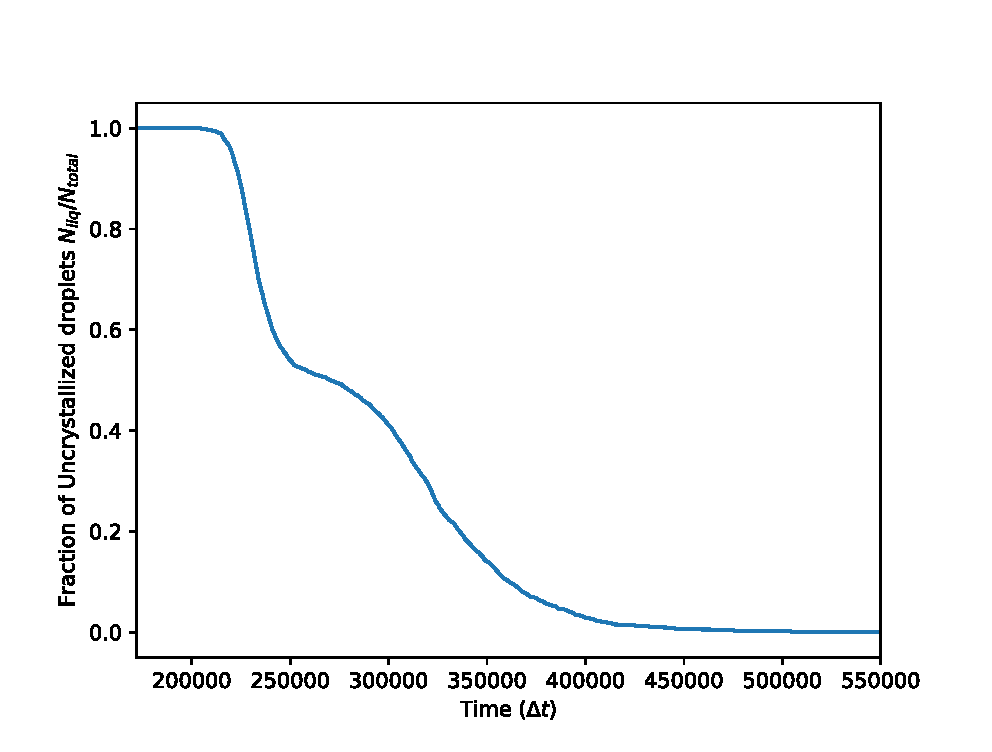
\includegraphics[width=\columnwidth]{incubation}
    \caption[Fraction of uncrystallized droplets in time]{
        \label{fig:incubation}
        Fraction of uncrystallized droplets in time.
    }
\end{figure}

%%%%%%%%%%%%%%%%%%%%%%%%%%%%%%%%%%%%%%%%%%%%%%%
\subsection{Outlook and Future Applications} %
%%%%%%%%%%%%%%%%%%%%%%%%%%%%%%%%%%%%%%%%%%%%%%%

The results presented here describe the behaviour of a quench followed by
multi-step precipitation process of relevance to the precipitation of gold
nano-particles observed in recent experiments. It is noteworthy that the
predicted results were done within a single framework and set parameters
corresponding to the improved XPFC alloy model introduced in this thesis. The
dynamical results shown here point to a richness in the landscape of kinetic
pathways to precipitation. One direction for future application of the improved
XPFC framework is to explore more of this landscape and to determine the effect
of quench parameter and solution concentration in nucleation kinetics, as well
as the polydispersity of precipitated particles, key features of interest to
experimental investigations of this topic.

\bibliography{references.bib}

\end{document}
